\documentclass[11pt,a4paper]{article}

\usepackage{amsmath,amssymb}
\usepackage{fontspec}
\usepackage{unicode-math}
\usepackage{polyglossia}
\setmainlanguage{french}
\usepackage{xcolor}
\usepackage{fancyhdr}
\usepackage[margin=2cm,headheight=16pt,headsep=22pt]{geometry}
\usepackage{tikz}
\usepackage{pgfplots}
\pgfplotsset{compat=1.18}
\usepackage{enumitem}
\usepackage{lastpage}

\IfFontExistsTF{Libertinus Serif}
  {\setmainfont{Libertinus Serif}}
  {\IfFontExistsTF{Latin Modern Roman}{\setmainfont{Latin Modern Roman}}{\setmainfont{lmroman10-regular.otf}}}

\IfFontExistsTF{Libertinus Math}
  {\setmathfont{Libertinus Math}}
  {\IfFontExistsTF{Latin Modern Math}{\setmathfont{Latin Modern Math}}{\setmathfont{latinmodern-math.otf}}}

\linespread{1.07}
\setlength{\parindent}{0pt}
\AtBeginDocument{\setlength{\parindent}{0pt}}
\setlength{\parskip}{0.35em}

\pagestyle{fancy}
\fancyhf{}
\lhead{NeoHarness AI -- Évaluation}
\rhead{Classe de Seconde}
\cfoot{Page \thepage\ / \pageref{LastPage}}
\renewcommand{\headrulewidth}{0.5pt}
\renewcommand{\headrule}{\vskip 5pt\hrule width\headwidth height\headrulewidth \vskip-\headrulewidth}

\setlist[enumerate,1]{itemsep=0.45em, topsep=0.3em, label=\textbf{\arabic*.}}
\setlist[enumerate,2]{itemsep=0.25em, topsep=0.2em, label=\textbf{\alph*.}}

\newcommand{\sujet}[1]{%
  \begin{center}%
    {\LARGE \textbf{ÉVALUATION DE MATHÉMATIQUES -- SUJET #1}}\\[0.4em]%
    {\large Nom : \makebox[4cm]{\dotfill} \quad Prénom : \makebox[4cm]{\dotfill} \quad Classe : \makebox[2cm]{\dotfill}}%
  \end{center}%
  \vspace{0.8em}%
}

\newcommand{\exo}[2]{%
  \vspace{1.2em}%
  \noindent{\large\textbf{Exercice #1. -- #2}}%
  \par\vspace{0.35em}%
  \hrule height 0.5pt%
  \vspace{0.7em}%
}

\newcommand{\partie}[1]{%
  \vspace{0.9em}%
  \noindent\textbf{#1}%
  \par\vspace{0.3em}%
}

\begin{document}

% ==================== SUJET A (ÉLÈVE) ====================
\sujet{A}

\exo{1}{Forme canonique, factorisation et extremum}
Soit $f$ la fonction définie sur $\mathbb{R}$ par l'expression :
$$f(x) = 2x^2 - 8x + 6$$
\begin{enumerate}
    \item Démontrer que pour tout réel $x$, on a : $f(x) = 2(x - 2)^2 - 2$.
    \item En déduire la factorisation de $f(x)$ en produit de deux facteurs du premier degré.
    \item Déterminer le minimum de la fonction $f$ sur $\mathbb{R}$ ainsi que la valeur de $x$ pour laquelle il est atteint.
    \item Résoudre dans $\mathbb{R}$ l'équation $f(x) = 6$.
    \item Dresser le tableau de variations complet de la fonction $f$ sur $\mathbb{R}$.
    \item Déterminer les coordonnées des points d'intersection de la courbe représentative de $f$ avec l'axe des abscisses.
    \item Calculer l'image de $0$ par la fonction $f$.
    \item Tracer schématiquement la parabole représentant $f$ en y faisant figurer son sommet et son axe de symétrie.
\end{enumerate}

\newpage

% ==================== SUJET B (ÉLÈVE ANTI-TRICHE) ====================
\sujet{B}

\exo{1}{Forme canonique, factorisation et extremum (Variante)}
Soit $g$ la fonction définie sur $\mathbb{R}$ par l'expression :
$$g(x) = 3x^2 + 12x + 9$$
\begin{enumerate}
    \item Démontrer que pour tout réel $x$, on a : $g(x) = 3(x + 2)^2 - 3$.
    \item En déduire la factorisation de $g(x)$ en produit de deux facteurs du premier degré.
    \item Déterminer le minimum de la fonction $g$ sur $\mathbb{R}$ ainsi que la valeur de $x$ pour laquelle il est atteint.
    \item Résoudre dans $\mathbb{R}$ l'équation $g(x) = 9$.
    \item Dresser le tableau de variations complet de la fonction $g$ sur $\mathbb{R}$.
    \item Déterminer les coordonnées des points d'intersection de la courbe représentative de $g$ avec l'axe des abscisses.
    \item Calculer l'image de $0$ par la fonction $g$.
    \item Tracer schématiquement la parabole représentant $g$ en y faisant figurer son sommet et son axe de symétrie.
\end{enumerate}

\newpage

% ==================== CORRIGÉS DÉTAILLÉS ====================
\begin{center}
  {\LARGE \textbf{CORRIGÉ OFFICIEL \& BARÈME}}\\[0.4em]
  {\large Sujet A et Sujet B}
\end{center}

\partie{Corrigé du Sujet A}
\begin{enumerate}
    \item \textbf{(1,25 pt)} On factorise par le coefficient dominant $2$ dans les deux premiers termes :
    $$f(x) = 2(x^2 - 4x) + 6$$
    On reconnaît le début de l'identité remarquable $(x-2)^2 = x^2 - 4x + 4$, soit $x^2 - 4x = (x-2)^2 - 4$.
    En remplaçant :
    $$f(x) = 2\left((x-2)^2 - 4\right) + 6 = 2(x-2)^2 - 8 + 6 = 2(x-2)^2 - 2$$
    \item \textbf{(1,25 pt)} À partir de la forme canonique :
    $$f(x) = 2\left[(x-2)^2 - 1\right] = 2\left[(x-2)^2 - 1^2\right] = 2(x - 2 - 1)(x - 2 + 1) = 2(x - 3)(x - 1)$$
    \item \textbf{(1 pt)} Le coefficient dominant est positif ($2 > 0$), donc la parabole est tournée vers le haut et admet un minimum. Le sommet est $S(2 ; -2)$. Le minimum est donc $-2$, atteint en $x = 2$.
    \item \textbf{(1,25 pt)} On résout $2x^2 - 8x + 6 = 6 \iff 2x^2 - 8x = 0 \iff 2x(x - 4) = 0$. Les solutions sont $x = 0$ et $x = 4$.
    \item \textbf{(1,25 pt)} La fonction est décroissante sur $]-\infty ; 2]$ puis croissante sur $[2 ; +\infty[$, avec un minimum de $-2$ en $2$.
    \item \textbf{(1,25 pt)} On résout $f(x) = 0 \iff 2(x-3)(x-1) = 0$, ce qui donne $x = 1$ et $x = 3$. Les points d'intersection sont $(1 ; 0)$ et $(3 ; 0)$.
    \item \textbf{(1 pt)} $f(0) = 2(0)^2 - 8(0) + 6 = 6$.
    \item \textbf{(1,25 pt)} Tracé de la parabole représentant $f$ :
    
    \begin{center}
    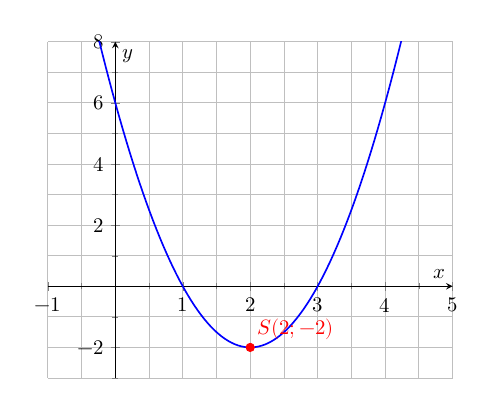
\begin{tikzpicture}[scale=0.75]
    \begin{axis}[
        xmin=-1, xmax=5,
        ymin=-3, ymax=8,
        axis lines=middle,
        xlabel=$x$,
        ylabel=$y$,
        grid=both,
        minor tick num=1,
        domain=-0.5:4.5,
        samples=100
    ]
    \addplot[blue, thick] {2*x^2 - 8*x + 6};
    \addplot[red, mark=*] coordinates {(2,-2)} node[above right] {$S(2;-2)$};
    \end{axis}
    \end{tikzpicture}
    \end{center}
\end{enumerate}

\vspace{1.5em}
\partie{Corrigé du Sujet B}
\begin{enumerate}
    \item \textbf{(1,25 pt)} On factorise par le coefficient dominant $3$ :
    $$g(x) = 3(x^2 + 4x) + 9$$
    On reconnaît $(x+2)^2 = x^2 + 4x + 4$, soit $x^2 + 4x = (x+2)^2 - 4$.
    $$g(x) = 3\left((x+2)^2 - 4\right) + 9 = 3(x+2)^2 - 12 + 9 = 3(x+2)^2 - 3$$
    \item \textbf{(1,25 pt)} À partir de la forme canonique :
    $$g(x) = 3\left[(x+2)^2 - 1\right] = 3(x + 2 - 1)(x + 2 + 1) = 3(x + 1)(x + 3)$$
    \item \textbf{(1 pt)} Le coefficient dominant est $3 > 0$, la parabole admet un minimum. Le sommet est $S(-2 ; -3)$. Le minimum est $-3$, atteint en $x = -2$.
    \item \textbf{(1,25 pt)} On résout $3x^2 + 12x + 9 = 9 \iff 3x^2 + 12x = 0 \iff 3x(x + 4) = 0$. Les solutions sont $x = 0$ et $x = -4$.
    \item \textbf{(1,25 pt)} La fonction est décroissante sur $]-\infty ; -2]$ puis croissante sur $[-2 ; +\infty[$, avec un minimum de $-3$ en $-2$.
    \item \textbf{(1,25 pt)} On résout $g(x) = 0 \iff 3(x+1)(x+3) = 0$, ce qui donne $x = -3$ et $x = -1$. Les points d'intersection sont $(-3 ; 0)$ et $(-1 ; 0)$.
    \item \textbf{(1 pt)} $g(0) = 3(0)^2 + 12(0) + 9 = 9$.
    \item \textbf{(1,25 pt)} Tracé de la parabole représentant $g$ :
    
    \begin{center}
    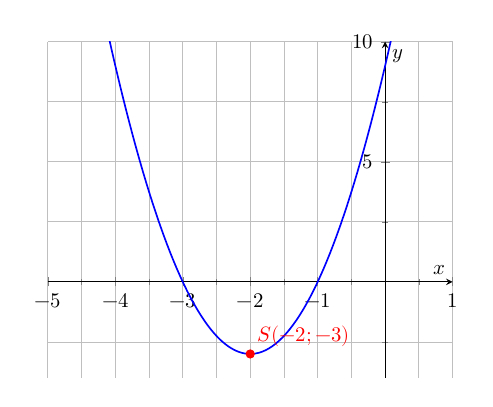
\begin{tikzpicture}[scale=0.75]
    \begin{axis}[
        xmin=-5, xmax=1,
        ymin=-4, ymax=10,
        axis lines=middle,
        xlabel=$x$,
        ylabel=$y$,
        grid=both,
        minor tick num=1,
        domain=-4.5:0.5,
        samples=100
    ]
    \addplot[blue, thick] {3*x^2 + 12*x + 9};
    \addplot[red, mark=*] coordinates {(-2,-3)} node[above right] {$S(-2;-3)$};
    \end{axis}
    \end{tikzpicture}
    \end{center}
\end{enumerate}

\end{document}